\chapter*{Introduction}
\addcontentsline{toc}{chapter}{Introduction}
\section{Contexte}

J'ai eu la chance d'effectuer mon stage au Laboratoire de Neurosciences-Cognitives de Marseille (LNC). Ce laboratoire constitue un centre de recherche de pointe dans les domaines des Neuroscience et de la Psychologie cognitive avec le Laboratoire de Psychologie Cognitive de Marseille (LPC). Ces deux laboratoires fusionneront pour former le CRPN, à partir de janvier 2024.

\vspace{2ex}
J'ai travaillé au sein de l'équipe de Développement Informatique et Infrastructure Système pour les Sciences du Cerveau (DI²S²C). Cette équipe de soutien à la recherche a deux missions principales. Tout d'abord, certaines membres s'occupent de la La gestion, l'administration et la maintenance de l’infrastructure informatique du centre de recherche. La deuxième mission consiste en la participation à des projets de recherche en apportant notamment une expertise en informatique scientifique (développement d'applications, conseils méthodologiques, calcul scientifique etc ...). L'équipe DI²S²C est dirigée par Jean-Luc Blanc, ingénieur de recherche CNRS, qui m'a acceuilli et guidé avec Anne-Sophie Dubarry, ingénieure de recherche CNRS dans la même équipe, pendant ces 6 mois. La structuration de cette équipe est détaillée par un organigramme en Figure \ref{fig0.1}. J'ai également eu l'opportunité d'échanger avec François-Xavier Alario, directeur de recherche CNRS au LPC, sur les aspects psyco-linguistiques que comprend mon travail, notamment dans les choix à effectuer pour la segmentation temporelle du signal et l'interprétation des résultats. J'ai aussi pu avoir le plaisir de travailler avec Laurent Pezard, professeur dans l'équipe Dynamique Auditive Neuronale (DNA) au LNC, et qui m'a beaucoup apporté en termes de compétence de développement informatique et de démarche scientifique.

\begin{figure}[!ht]
    \centering
    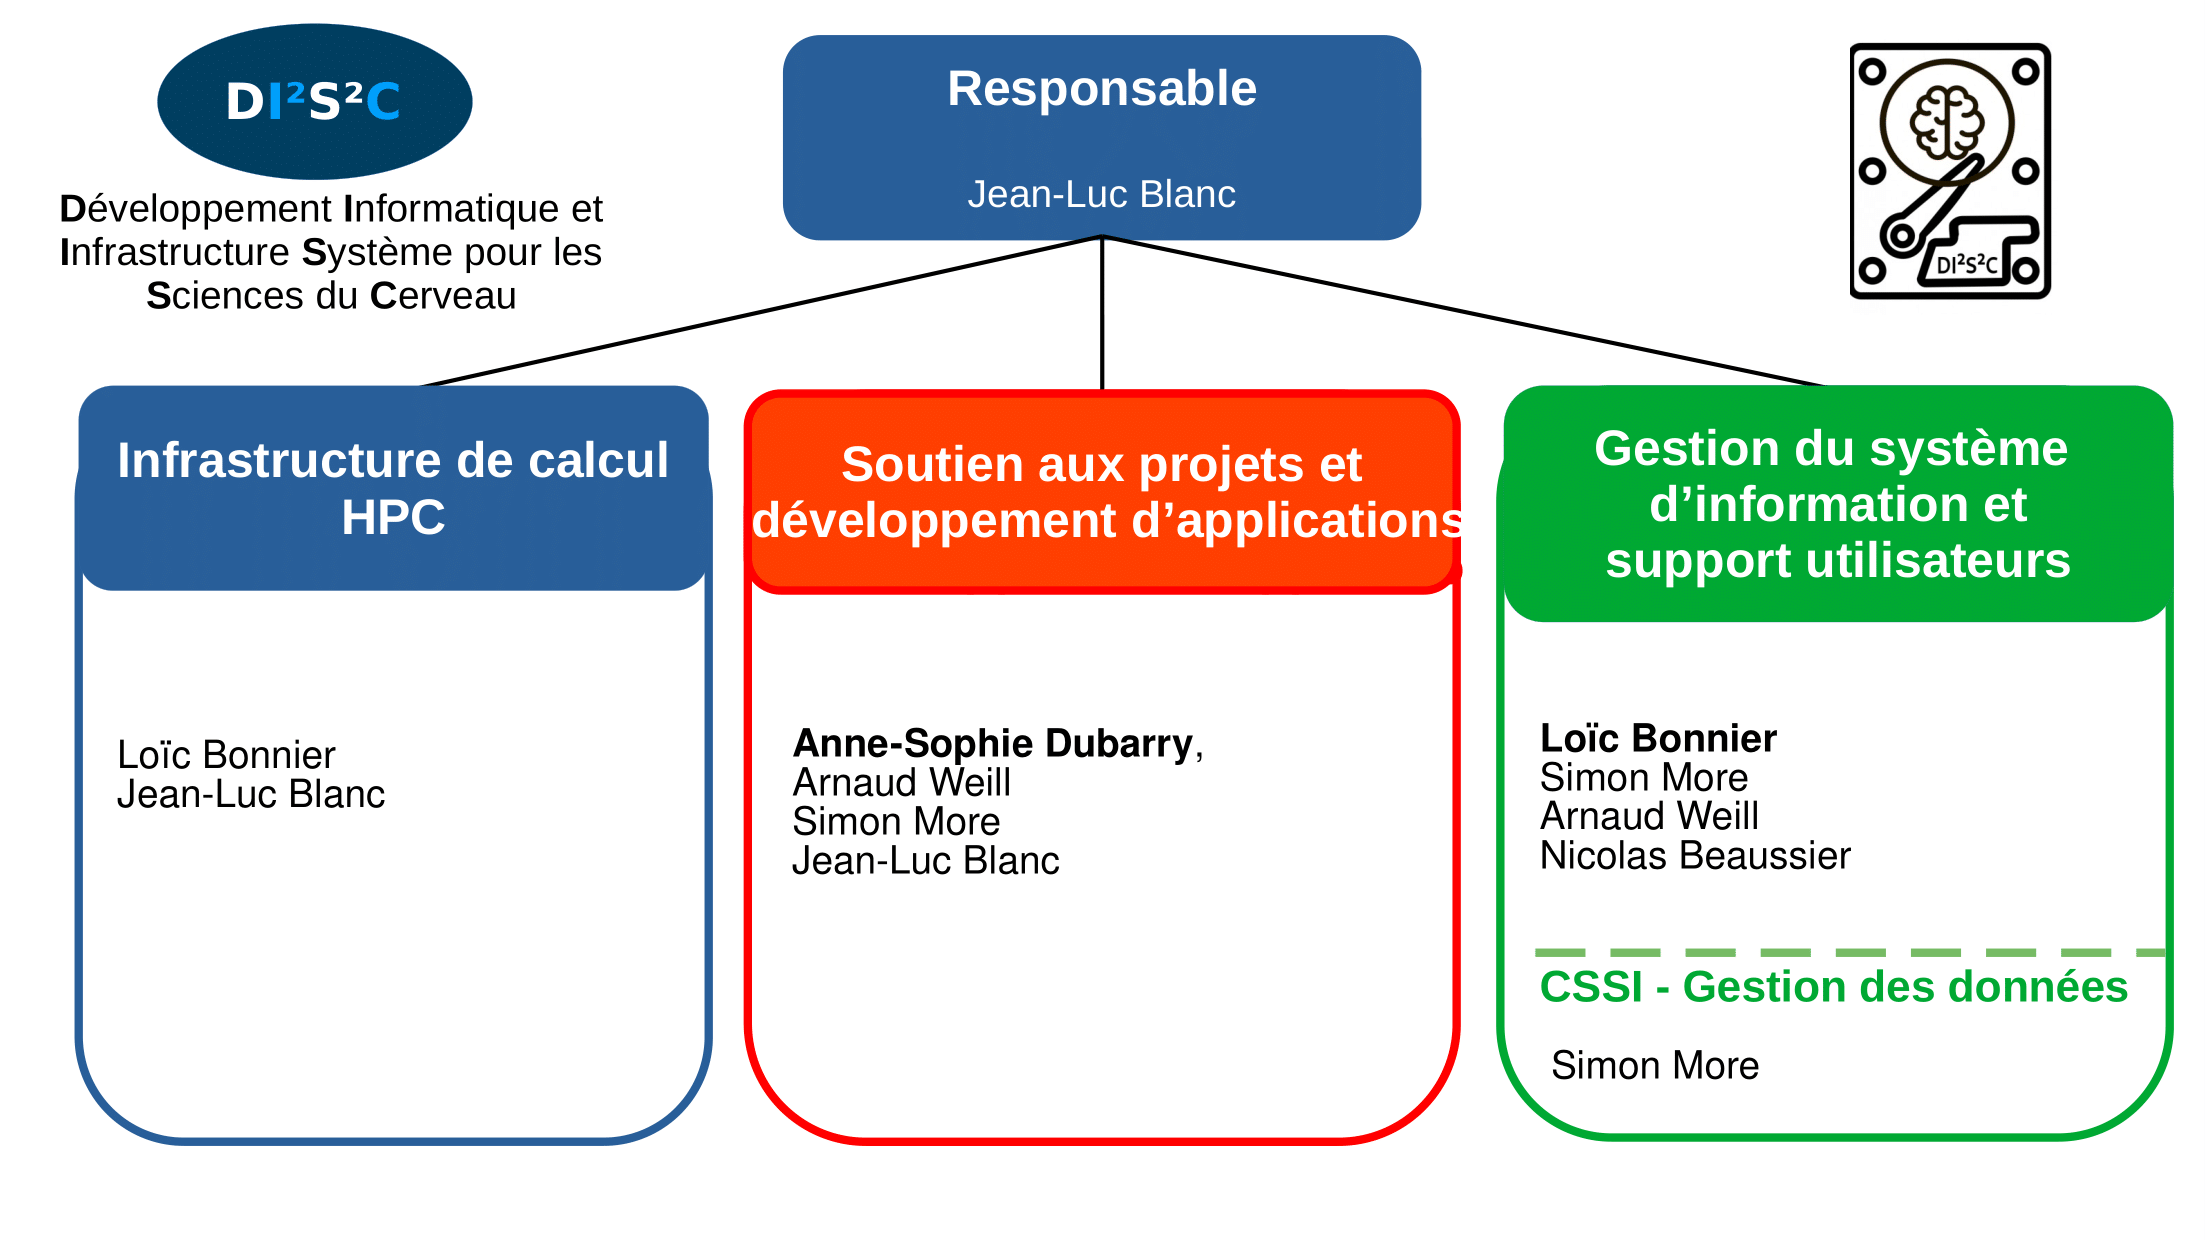
\includegraphics[width=13cm]{OrganigrameDISC.png}
    \caption{Organigrame de l'équipe DISC}
    \label{fig0.1}
\end{figure} 

\section{Objectifs du stage}

Durant ce stage, nous avions pour ambition de faire le lien entre complexité linguistique et la dynamique cérébrale. Que se passe-t-il dans le cerveau, en termes d'activation de population de neurones, lorsqu'une personne comprend, ou non, une phrase qu'elle lit ou qu'elle entend ?
La compréhension linguistique, qu’elle soit orale ou écrite, passe par la capacité à combiner des mots d’une phrase pour en saisir le sens; Qui a fait quoi ? A qui ? Ce n’est pas une simple concaténation. On s’intéresse donc à la dynamique cérébrale, au processus d’opérations cognitives qui permet la compréhension de chaque mot et de leur sémantique ainsi que la syntaxe et le contexte dans lesquels ils sont inscrits pour comprendre le sens de la phrase. 

Le point de départ de mon travail repose sur des enregistrements des champs magnétiques émis par le cerveau de par son activité (signal magnétoencéphalographique ou MEG). Ces données constituent une mesure de la dynamique cérébrale que j'ai étudié. L'objectif de mon stage était donc de mettre en place un algorithme permettant d'extraire des représentations symboliques à partir de segments des séries temporelles du signal MEG (Figure \ref{fig0.2}), découpées en fonction des différents stimuli. Ces stimulis correspondent à différents degrés de complexité linguistique. Par exemple, on peut s'intéresser à comparer l'activité cérébrale lors de la lecture ou de l'écoute de phrases simples par rapport à celle lors de phrases complexes au sens grammatical. On se focalisera sur la dynamique cérébrale liée à la compréhension de chaque mot d'une phrase. Ces représentations symboliques permettent de représenter un système dynamique continu (le cerveau) comme une séquence de symboles correspondants à des états discrets du système étudié. En effet, on se base sur l'espace des phases (ou espace des états) \cite{18} qui constitue l'espace mathématique dans lequel tous les états possibles du système sont représentés ; chaque état possible correspond à un point unique dans l'espace des phases. Cet espace permet de nous affranchir du temps en représentant les capteurs les uns en fonction des autres dans un hyperespace, où chacun d'eux représente un degré de liberté du système dynamique étudié. La représentation symbolique est une méthode qui permet d'associer un symbole à chaque partie de l'espace des phases en regard d'une partition comme illustré en (c) de la Figure \ref{0.2}. On a alors des séquences de symboles que l'on appelle séquences symboliques qui rendent compte de la dynamique cérébrale. En effet, chaque symbole correspond alors à un ou plusieurs états possibles (en fontion de la finesse de la partition) du système dynamique étudié. Cela permet de rendre compte de la complexité intrinsèque de la dynamique cérébrale et de la quantité d'information contenue dans celle-ci grâce à une métrique puissante : l'entropie.

\begin{figure}[!ht]
    \centering
    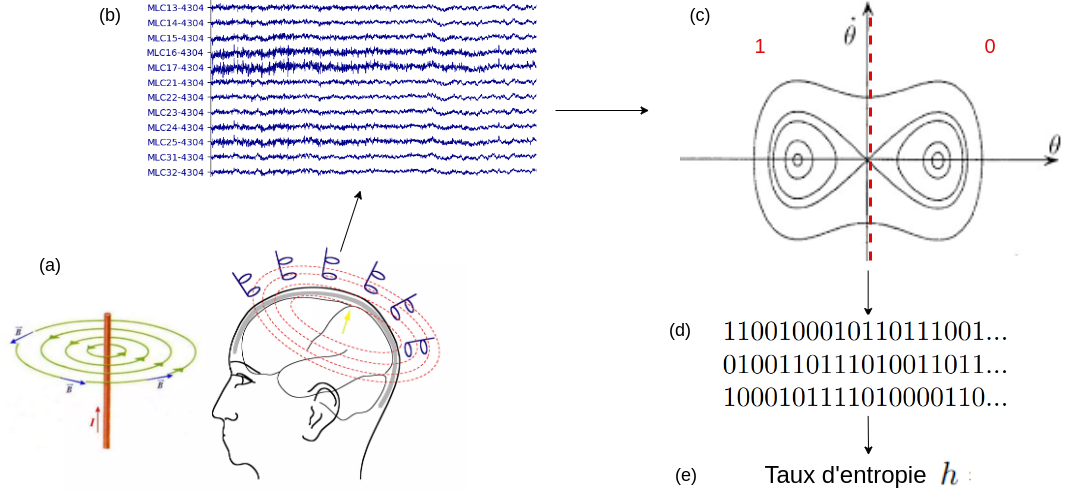
\includegraphics[width=17cm]{schema_algorithme.png}
    \caption{Schéma de l'algorithme mis en place durant le stage. (a) Mesure des champs magnétiques générés de par l'activité cérébrale. (b) Séries temporelles des capteurs. (c) Représentation symbolique de l'espace des phases des capteurs avec à une partition. Ici représenté en seulement 2 dimenions avec une partition binaire, les points des trajectoires à gauche de la ligne en pointillé rouge sont associées au symbole 1 tandis que ceux à droite au symbole 0. (d) Séquences symboliques représentées pour chaque capteur. (e) Taux d'entropie de chaque séquence symbolique.}
    \label{fig0.2}
\end{figure}

Le but est donc de calculer l'entropie de représentations symboliques associées à des conditions expérimentales et de les comparer entre elles. De cette manière, on lie la complexité linguistique et sa compréhension à la dynamique cérébrale associée. Cette métrique qu'est l'entropie est définie à l'intersection de 3 domaines. Dans le cadre de la théorie de l'information, l'entropie mesure la quantité d'information du signal d'origine qui a été produite par une source. Dans le cadre de la théorie des systèmes dynamiques, cette quantité rend compte de la complexité intrinsèque du système dynamique étudié en lien avec les notions d'ordre et de désordre. Enfin, dans le cadre de l'informatique théorique, l'entropie indique de la complexité du codage de la séquence symbolique permettant de décrire un phénomène observé par rapport à un alphabet universel. L'entropie est donc un indicateur, une métrique, qui nous renseigne sur la dynamique du système complexe que l'on étudie : le cerveau. Dans le cadre de cette étude, l'entropie nous permet donc mesurer l'effet de la complexité linguistique sur l'activité neuronale et de rendre compte de la dynamique cérébrale sous-jacente associée à la compréhension. 

La problématique de mon stage est donc la suivante : Peut-on discriminer des conditions expérimentales et rendre compte d'une compréhension linguistique sur la base de la quantification précise de la dynamique cérébrale ?

\vspace{2ex}
J'étudierai dans un premier temps l'origine neurophysiologique et les techniques d'enregistrement des signaux sur lesquelles nous travaillons avant d'introduire la base de données MEG que nous avons utilisée pour cette étude. J'expliquerai ensuite le processus de pré-traitement du signal MEG ainsi que la segmentation temporelle de celui-ci en regard des conditions expérimentales. Puis, je présenterai les concepts et les méthodes de la théorie de l'information et de la théorie des systèmes dynamiques que nous avons utilisé pour notre algorithme. Je me focaliserai principalement sur la représentation symbolique d'un système dynamique et l'entropie d'une séquence symbolique. Enfin, je détaillerai l'implémentation de l'algorithme mis en place au cours du stage et les résultats obtenus à partir des données expérimentales.

